% =====================================================================================
% PROTOCOLE D'ELICITATION -- version 2, 13 aout 2026
%
% CE QUI A CHANGE. Cette piece est celle qu'un relecteur juge, et cinq points la rendaient
% contestable en l'etat :
%  1. la table des graines annoncait « xi = 0,90 » comme valeur vraie. C'est la valeur POSEE du
%     pire cas, pas la calibration figee (0,5954). La graine est RETIREE, pas corrigee, car xi
%     est une estimation d'IC90 [0,30 ; 0,83] et une graine doit avoir une valeur realisee ;
%  2. quatre graines venaient de scripts dont la sortie n'etait pas versionnee, donc leur
%     valeur vraie n'etait verifiable par personne. Les sorties 08e et 08f sont desormais
%     versionnees et les neuf graines sont toutes reproductibles ;
%  3. la convention de direction etait INVERSEE par rapport au memoire (« de k vers j » quand le
%     memoire ecrit W_jk avec j la source). Une saisie fidele aurait transpose W ;
%  4. le protocole promettait que les intervalles elicites « bornent le SCR », ce qui contredit
%     le gel de la calibration du 7 aout. L'elicitation est un AXE DE SENSIBILITE declare ;
%  5. il nommait quatre collaborateurs reels, dont un ayant quitte le projet, et la figure de
%     demonstration attachait a des prenoms reels des profils « sur-confiant » et « biaise ».
% =====================================================================================
\documentclass[11pt,a4paper]{article}

\usepackage[utf8]{inputenc}
\usepackage[T1]{fontenc}
\usepackage{lmodern}
\usepackage[french]{babel}
\usepackage[margin=2.0cm]{geometry}
\usepackage{microtype}
\usepackage{booktabs}
\usepackage{array}
\usepackage[table]{xcolor}
\usepackage{amsmath}
\usepackage{graphicx}
\usepackage{caption}
\usepackage[most]{tcolorbox}
\usepackage{fancyhdr}
\usepackage{lastpage}

\definecolor{navy}{HTML}{1F3864}
\definecolor{lightblue}{HTML}{D6E0F0}
\definecolor{softgray}{HTML}{F2F2F2}

\captionsetup{font=small,labelfont={bf,color=navy},labelsep=period}
\graphicspath{{../../vasicek_lab/figures/}}

\newtcolorbox{cle}[1][]{colback=lightblue!40,colframe=navy,boxrule=0.6pt,
  arc=2pt,left=8pt,right=8pt,top=6pt,bottom=6pt,#1}
\newtcolorbox{garde}[1][]{colback=softgray,colframe=black!40,boxrule=0.5pt,
  arc=2pt,left=8pt,right=8pt,top=6pt,bottom=6pt,#1}

\pagestyle{fancy}
\fancyhf{}
\lfoot{\footnotesize Protocole d'élicitation $W$ --- version 2.0 du 13 août 2026}
\rfoot{\footnotesize page \thepage/\pageref{LastPage}}
\renewcommand{\headrulewidth}{0pt}

\title{\vspace{-1.3cm}\color{navy}\bfseries Protocole d'élicitation de $W$\\[2pt]
  \large Méthode de Cooke, étalonnée sur les faits mesurés de l'étude}
\author{Kélian Kaddouri --- mémoire d'actuariat, ENSAE Paris / Institut des Actuaires}
\date{Version 2.0 --- 13 août 2026}

\begin{document}
\maketitle
\thispagestyle{fancy}
\vspace{-0.6cm}

\begin{cle}
\textbf{Pourquoi une élicitation.} La matrice de contagion dirigée $W$ entre les cinq piliers
n'est pas calibrable sur les données disponibles : la co-occurrence de deux défaillances est
observable, leur \emph{ordre} ne l'est pas. Plutôt qu'un dire d'expert brut, on l'obtient par une
élicitation \textbf{pondérée par la performance} (Cooke, 1991) : les répondants sont notés sur des
questions à réponse connue, et leur influence sur $W$ est proportionnelle à leur \emph{justesse}
et à leur \emph{finesse}. Le résultat est un $W$ auditable et assorti d'une \textbf{incertitude},
et non un jeu de coefficients affirmés.
\end{cle}

\begin{garde}
\textbf{Statut de cette pièce, à lire avant le reste.} Le protocole est \textbf{préparé et non
exécuté}. La calibration de l'étude est \textbf{gelée} depuis le 7 août 2026 : une élicitation
menée aujourd'hui ne remplacerait donc aucun résultat publié et ne déplacerait aucun capital. Elle
constituerait un \textbf{axe de sensibilité déclaré}, à comparer aux bornes d'identification
partielle qui tiennent lieu de référence, et c'est sous ce statut que ses résultats seraient
présentés. Ce point est décisif pour un relecteur : ce document ne demande pas d'accréditer une
recalibration, mais un instrument de mesure de l'incertitude.
\end{garde}

\subsection*{La méthode, en quatre temps}
\begin{itemize}\itemsep2pt
\item \textbf{Format.} Chaque quantité est élicitée en trois quantiles, $5\,\%$, $50\,\%$ et
      $95\,\%$, soit un intervalle de crédibilité et non un point.
\item \textbf{Calibration.} Sur les questions-graines, à réponse connue de l'analyste, on teste
      si les réalisations tombent dans les bandes annoncées aux fréquences attendues
      ($5/45/45/5\,\%$). Le score est la $p$-value d'un $\chi^2$ ; il s'effondre pour un
      répondant sur-confiant ou biaisé.
\item \textbf{Information.} Finesse des intervalles, mesurée par la divergence de
      Kullback-Leibler à un fond uniforme, sur une plage \emph{commune} à tous les répondants.
      Un répondant vague est peu informatif.
\item \textbf{Poids et agrégation.} Poids $=$ calibration $\times$ information, nul sous le seuil
      $\alpha=0{,}05$. Le décideur est le mélange linéaire pondéré des répondants sur les liens
      cibles de $W$.
\end{itemize}

\subsection*{Les neuf questions-graines, et ce qui les rend défendables}

Une graine sert à \emph{noter} un répondant : sa valeur vraie doit donc être une grandeur
\textbf{réalisée}, mesurée sur les données, et \textbf{reproductible}. Les neuf retenues le sont
toutes, chacune par une sortie de script versionnée, référencée ci-dessous.

\begin{center}\footnotesize
\renewcommand{\arraystretch}{1.12}
\begin{tabular}{@{}p{10.4cm} r l@{}}
\toprule
\textbf{Question-graine} & \textbf{Valeur} & \textbf{Source} \\
\midrule
Part des sinistres financiers portés par une cause commune (tiers) & $20\,\%$ & \texttt{08g} \\
Délai médian entre survenance et déclaration & $94$ j & \texttt{08e} \\
Part des incidents déclarés après un mois & $85\,\%$ & \texttt{08e} \\
Durée médiane de brèche (\emph{containment}) & $7$ j & \texttt{08f} \\
Fréquence d'incidents TIC matériels, entité de grande taille, par an & $0{,}21$ & \texttt{08b} \\
Délai médian de déclaration d'un incident de type piratage & $117$ j & \texttt{08e} \\
Indice de Gini de la concentration journalière & $0{,}69$ & \texttt{08g} \\
Nombre maximal de victimes d'une cause commune en un jour & $191$ & \texttt{08g} \\
Part des jours qui portent une cause commune & $1{,}7\,\%$ & \texttt{08g} \\
\bottomrule
\end{tabular}
\end{center}

\vspace{4pt}
\begin{garde}
\textbf{Une dixième graine a été retirée, et le dire vaut mieux que le taire.} La version de
juillet comptait une question sur l'indice de queue de sévérité $\xi$, avec pour valeur vraie
$0{,}90$. Deux défauts s'y cumulaient. D'abord $0{,}90$ n'est pas la calibration mais la valeur
\emph{posée} du scénario de pire cas ; la calibration figée donne $\xi=0{,}5954$. Or dans la
méthode de Cooke une graine fausse ne dégrade pas le résultat à la marge : elle \textbf{inverse}
les poids, en pénalisant le répondant qui vise juste. Ensuite, et c'est la raison du retrait
plutôt que de la correction, $\xi$ est une \emph{estimation} assortie d'un intervalle à $90\,\%$
de $[0{,}30\,;0{,}83]$, plus large que la valeur elle-même : noter quiconque contre un tel nombre
n'a pas de sens. Une graine doit être une réalisation, pas un paramètre estimé.
\end{garde}

\subsection*{Les questions cibles, et la convention de direction}

\begin{garde}
\textbf{Convention, à vérifier avant toute saisie.} On élicite $W_{jk}$, force du lien dirigé
allant de $j$ vers $k$, où \textbf{$j$ est le pilier qui défaille en premier} et $k$ celui qui est
entraîné. C'est la convention de l'étude : \emph{la ligne émet, la colonne reçoit}. Le formulaire
de juillet notait ces liens \og de $k$ vers $j$ \fg, soit l'ordre inverse des lettres : une saisie
fidèle à ce formulaire aurait \textbf{transposé} $W$, donc inversé toutes les conclusions de
direction. Les deux sens d'une même paire sont élicités séparément et n'ont aucune raison d'être
égaux, l'asymétrie étant précisément l'objet de la mesure.
\end{garde}

\vspace{4pt}
\noindent Six liens sont élicités : P1$\to$P2 et P2$\to$P1, qui portent la question d'asymétrie,
puis P4$\to$P2, P1$\to$P4, P3$\to$P1 et P5$\to$P2, que le corpus documentaire atteste. Le modèle
en compte vingt ; les quatorze autres restent bornés par l'identification partielle, et les
éliciter serait une extension du même formulaire, sans changement de méthode.

\begin{center}
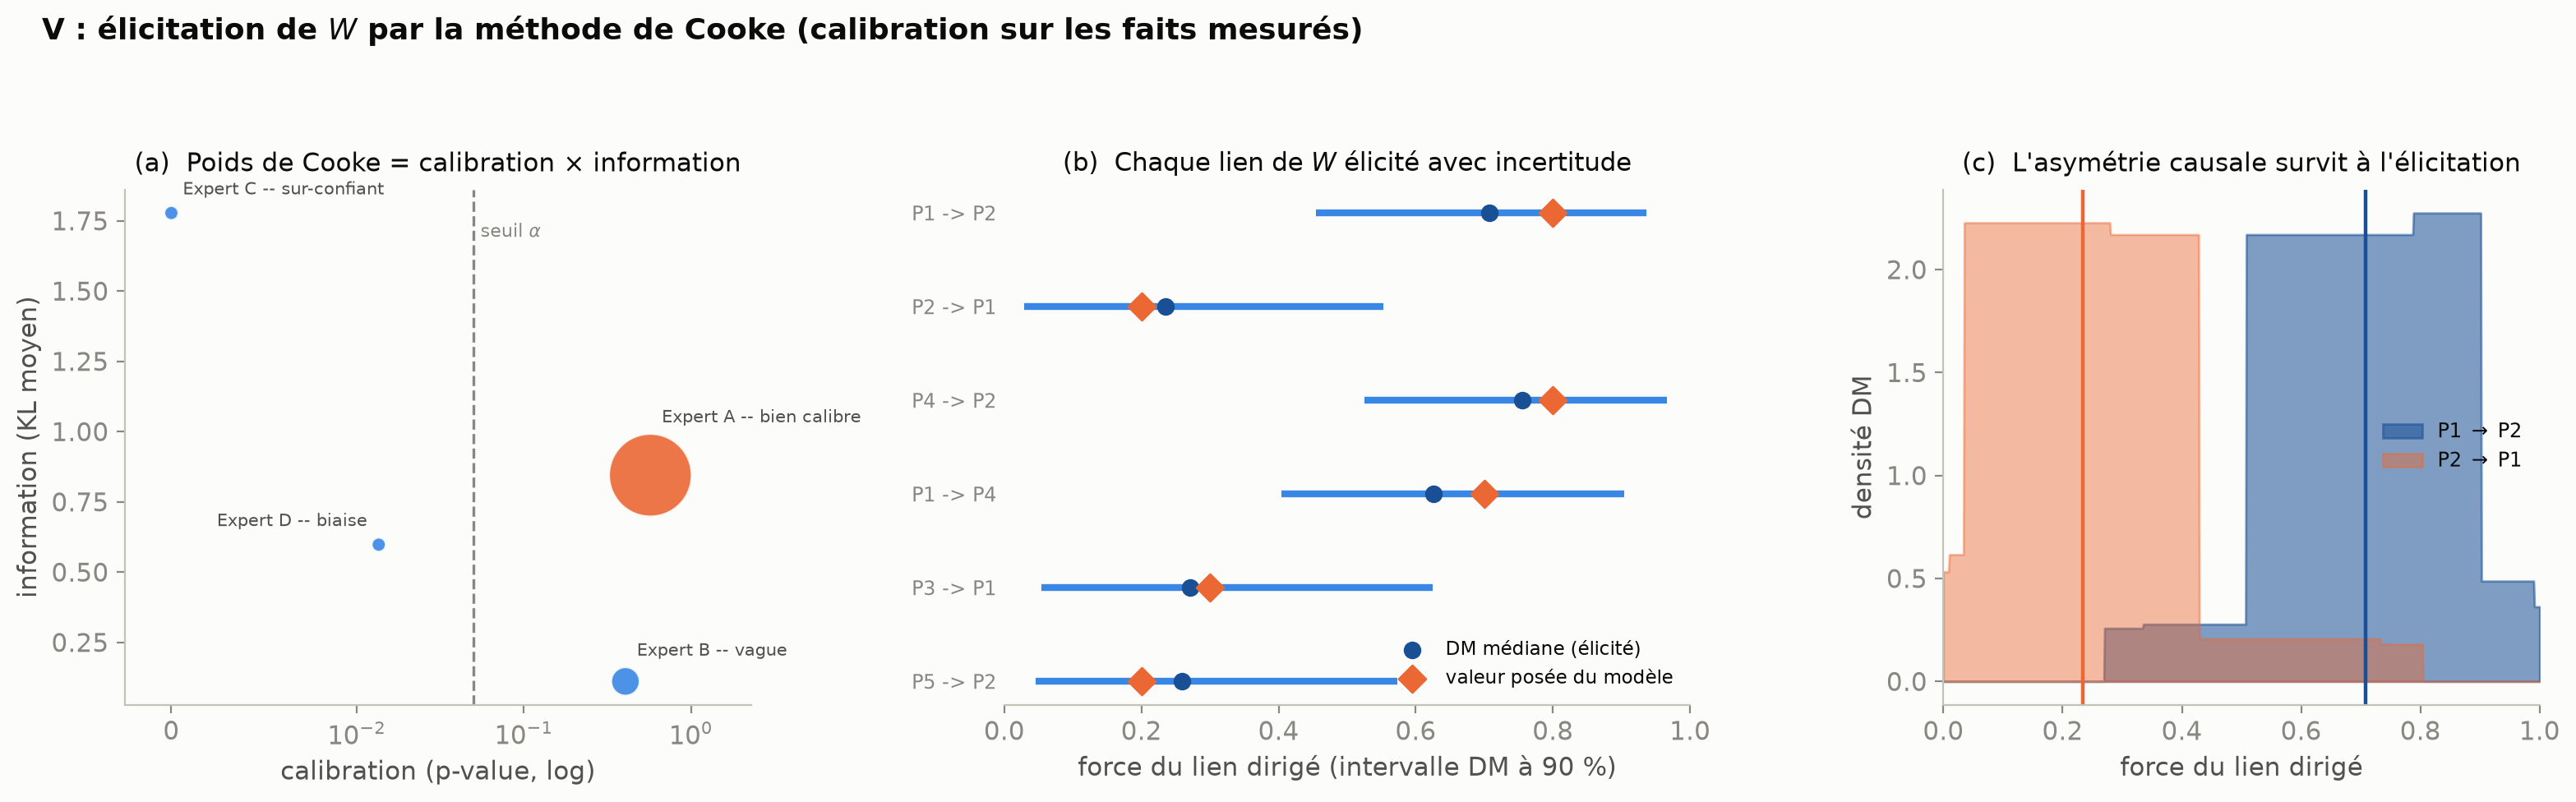
\includegraphics[width=\linewidth]{V_elicitation_cooke.png}
\captionof{figure}{Démonstration sur des répondants \textbf{fictifs} de profils contrastés, sur
les neuf graines retenues. \textbf{(a)}~le profil bien calibré et informatif domine
($91{,}5\,\%$ du poids) ; le sur-confiant et le biaisé passent sous le seuil $\alpha$ et sont
écartés. \textbf{(b)}~chaque lien de $W$ ressort avec un intervalle à $90\,\%$, comparé à la
valeur posée du modèle. \textbf{(c)}~l'asymétrie entre P1$\to$P2 et P2$\to$P1 survit à
l'élicitation. Les profils sont anonymes et décrivent un comportement, non une personne.}
\end{center}

\subsection*{Conduite d'une séance, et traitement}

\begin{itemize}\itemsep2pt
\item \textbf{Un répondant à la fois}, sans échange entre eux : des réponses qui se ressemblent
      parce qu'elles ont été discutées vident la pondération de Cooke de son sens.
\item \textbf{Ordre des trois nombres} : la haute d'abord, la basse ensuite, la médiane en
      dernier. Demander la médiane en premier ancre les deux autres et resserre artificiellement
      les intervalles, seul biais que la méthode sanctionne réellement.
\item \textbf{Aucun chiffre soufflé}, aucune réaction à une réponse : le moindre signal ancre.
      L'antisèche d'animation jointe détaille les relances neutres et ce qu'il faut bannir.
\item \textbf{Traitement} par \texttt{26\_elicitation\_cooke.py} (moteur et démonstration) puis
      \texttt{26b\_elicitation\_reelle.py} (réponses réelles). Les réponses sont saisies sous
      identifiant anonyme dans \texttt{elicitation\_reponses.csv}.
\end{itemize}

\begin{cle}
\textbf{Ce qu'il reste à faire, et ce que cela coûte.} Le moteur, le questionnaire, l'antisèche et
le gabarit de saisie sont prêts et vérifiés. Il reste à faire répondre les experts, à saisir leurs
réponses et à lire les poids et le $W$ élicité avec ses intervalles. Aucune donnée d'incident
n'est requise, seulement du temps d'expert, de l'ordre de trente minutes par répondant. La
décision de lancer ou non l'élicitation est donc \textbf{réversible sans coût de développement},
et c'est cette réversibilité que la présente version rend effective.
\end{cle}

\end{document}
